\documentclass[12pt,a4paper]{article}
\usepackage[utf8]{inputenc}
\usepackage[T1]{fontenc}
\usepackage{german}
\usepackage{amsmath, amssymb, amsthm}
\usepackage{physics}
\usepackage{siunitx}
\usepackage{tikz}
\usetikzlibrary{arrows.meta, decorations.pathmorphing, decorations.markings,
                patterns, calc, positioning, shapes.geometric, angles, quotes,
                decorations.pathreplacing, backgrounds, shadings, fadings}
\usepackage{pgfplots}
\pgfplotsset{compat=1.18}
\usepackage{booktabs}
\usepackage{array}
\usepackage{multirow}
\usepackage{geometry}
\usepackage{xcolor}
\usepackage{hyperref}
\usepackage{float}
\usepackage{caption}
\usepackage{subcaption}
\usepackage{enumitem}
\usepackage{fancyhdr}
\usepackage{titlesec}
\usepackage{mathtools}
\usepackage{bm}

\geometry{a4paper, left=2.5cm, right=2.5cm, top=3cm, bottom=3cm}

% ---- Farben ----
\definecolor{hyprot}{RGB}{180,30,20}
\definecolor{hypblau}{RGB}{15,50,120}
\definecolor{schockgelb}{RGB}{220,160,10}
\definecolor{plasmaviolett}{RGB}{120,30,160}
\definecolor{ablgruen}{RGB}{30,120,60}
\definecolor{hellgrau}{RGB}{235,235,240}
\definecolor{dunkelgrau}{RGB}{70,70,80}
\definecolor{hitzeorange}{RGB}{210,90,20}

\hypersetup{colorlinks=true, linkcolor=hypblau, citecolor=hypblau, urlcolor=hypblau,
  pdftitle={Hyperschallaerodynamik im zivilen Kontext}}

\newtheorem{satz}{Satz}[section]
\newtheorem{definition}{Definition}[section]
\newtheorem{herleitung}{Herleitung}[section]
\newtheorem{bemerkung}{Bemerkung}[section]

% ---- Makros ----
\newcommand{\Ma}{M\!a}
\newcommand{\Rey}{Re}
\newcommand{\Dv}{\Delta v}
\newcommand{\vek}[1]{\boldsymbol{#1}}
\newcommand{\tensor}[1]{\underline{\underline{#1}}}

% ======================================================
\title{Strömungsmechanik und Hyperschallaerodynamik\\[0.4em]
  \large\textit{Im zivilen Kontext: Raumgleiter, Wiedereintrittsfahrzeuge\\
und atmosph\"{a}rische Hochgeschwindigkeitsflugk\"{o}rper}}
\author{Stephan Epp}
\date{\today}

\begin{document}
% ======================================================

% ---- Titelseite ----
\maketitle

\tableofcontents
\newpage

%=======================================================
\section{Einleitung: Das Hyperschallregime}
%=======================================================

Hyperschall bezeichnet Strömungen mit Machzahlen $\Ma \geq 5$. In diesem Regime
treten physikalische Phänomene auf, die in der klassischen Unterschall- und
Überschallaerodynamik keine Rolle spielen: extreme Aerothermodynamik,
Dissoziation und Ionisation der Luft, dominante Viskositätseffekte und starke
Interaktionen zwischen Stoßwellen und Grenzschichten.

Für den zivilen Raumfahrtbereich ist das Hyperschallregime unausweichlich: Jedes
Fahrzeug, das aus dem Orbit oder von einer suborbitalen Bahn in die Erdatmosphäre
eintritt, durchquert dieses Regime. Die Mission des Space Shuttle, der Apollo-Kapsel,
der Sojus-Kapsel, des SpaceX Dragon sowie zukünftiger Konzepte wie dem Raumgleiter
Hermes oder der IXV-Demonstratorkonfiguration der ESA basieren sämtlich auf der
Beherrschung der Hyperschallphysik.

\begin{definition}[Machzahl und Strömungsregime]
Die \textbf{Machzahl} ist definiert als Verhältnis der lokalen Strömungsgeschwindigkeit
$v$ zur lokalen Schallgeschwindigkeit $a$:
\[
  \Ma = \frac{v}{a}, \qquad a = \sqrt{\gamma R T}
\]
Einteilung der Strömungsregime:
\[
  \Ma < 1 \text{ (Unterschall)},\quad
  1 \leq \Ma < 5 \text{ (Überschall)},\quad
  \Ma \geq 5 \text{ (Hyperschall)}
\]
Bei Wiedereintritt aus LEO: $\Ma \approx 25$; Apollo-Wiedereintritt: $\Ma \approx 33$.
\end{definition}

%=======================================================
\section{Grundgleichungen der kompressiblen Strömungsmechanik}
%=======================================================

\subsection{Navier-Stokes-Gleichungen in Kompressibilität}

Die Bewegungsgleichungen für ein kompressibles, viskoses Fluid lauten in
Indexschreibweise (Einsteinsche Summenkonvention):

\begin{align}
  \frac{\partial \rho}{\partial t} + \frac{\partial (\rho u_i)}{\partial x_i} &= 0
  \tag{Kontinuität}\label{eq:kont}\\[4pt]
  \frac{\partial (\rho u_i)}{\partial t} + \frac{\partial (\rho u_i u_j)}{\partial x_j}
  &= -\frac{\partial p}{\partial x_i} + \frac{\partial \tau_{ij}}{\partial x_j} + \rho g_i
  \tag{Impuls}\label{eq:impuls}\\[4pt]
  \frac{\partial (\rho E)}{\partial t} + \frac{\partial [(\rho E + p)u_i]}{\partial x_i}
  &= \frac{\partial (u_j \tau_{ij})}{\partial x_i}
    - \frac{\partial q_i}{\partial x_i} + \dot{Q}
  \tag{Energie}\label{eq:energie}
\end{align}

Der viskose Spannungstensor für ein Newton'sches Fluid:
\[
  \tau_{ij} = \mu\left(\frac{\partial u_i}{\partial x_j}
    + \frac{\partial u_j}{\partial x_i}\right)
    - \frac{2}{3}\mu\,\delta_{ij}\frac{\partial u_k}{\partial x_k}
\]

Die Gesamtenergie pro Masseneinheit: $E = e + \frac{1}{2}u_i u_i$, wobei $e$ die
innere Energie ist. Der Wärmestromvektor folgt dem Fourier'schen Gesetz:
$q_i = -\lambda\,\partial T/\partial x_i$.

\subsection{Isentrope Strömungsbeziehungen}

Für eine reibungsfreie, adiabate (isentrope) Strömung gelten die
Isentropenbeziehungen zwischen Staupunktzustand ($\cdot_0$) und lokalem Zustand:

\begin{satz}[Isentrope Zustandsgrößen]
\begin{align}
  \frac{T_0}{T} &= 1 + \frac{\gamma-1}{2}\Ma^2
  \label{eq:T_isentrop}\\[4pt]
  \frac{p_0}{p} &= \left(1 + \frac{\gamma-1}{2}\Ma^2\right)^{\gamma/(\gamma-1)}
  \label{eq:p_isentrop}\\[4pt]
  \frac{\rho_0}{\rho} &= \left(1 + \frac{\gamma-1}{2}\Ma^2\right)^{1/(\gamma-1)}
  \label{eq:rho_isentrop}
\end{align}
Für $\Ma = 25$ und $\gamma = 1.4$ (kalt, ohne Dissoziation):
$T_0/T = 1 + 0.2 \times 625 = 126 \quad\Rightarrow\quad T_0 = 126\,T_\infty$.
\end{satz}

\subsection{Senkrechter Verdichtungsstoß (Normal Shock)}

An senkrechten Verdichtungsstößen gelten die Rankine-Hugoniot-Bedingungen.
Sei $\Ma_1$ die Machzahl vor dem Stoß:

\begin{herleitung}[Rankine-Hugoniot-Sprungbedingungen]
Aus Erhaltung von Masse, Impuls und Energie über die Stoßfront ($\perp$ zur Stoßfläche):
\begin{align*}
  \rho_1 u_1 &= \rho_2 u_2 \tag{Masse}\\
  p_1 + \rho_1 u_1^2 &= p_2 + \rho_2 u_2^2 \tag{Impuls}\\
  h_1 + \tfrac{1}{2}u_1^2 &= h_2 + \tfrac{1}{2}u_2^2 \tag{Energie}
\end{align*}
Mit $h = \gamma p / [(\gamma-1)\rho]$ folgt nach Elimination:
\[
  \boxed{\Ma_2^2 = \frac{\Ma_1^2 + \frac{2}{\gamma-1}}{\frac{2\gamma}{\gamma-1}\Ma_1^2 - 1}}
  \qquad
  \frac{\rho_2}{\rho_1} = \frac{(\gamma+1)\Ma_1^2}{(\gamma-1)\Ma_1^2 + 2}
  \qquad
  \frac{p_2}{p_1} = \frac{2\gamma\Ma_1^2 - (\gamma-1)}{\gamma+1}
\]
Für $\Ma_1 \to \infty$ (Hyperschall-Grenzfall):
\[
  \frac{\rho_2}{\rho_1} \to \frac{\gamma+1}{\gamma-1}
    \underset{\gamma=1.4}{=} 6, \qquad
  \frac{p_2}{p_1} \to \frac{2\gamma}{\gamma+1}\Ma_1^2, \qquad
  \frac{T_2}{T_1} \to \frac{2\gamma(\gamma-1)}{(\gamma+1)^2}\Ma_1^2
\]
Die \emph{Dichtegrenze} bei 6 ist charakteristisch für Hyperschall --- die
Strömung kann sich trotz beliebig hoher Machzahl nur bis zum Faktor 6 verdichten
(für $\gamma = 1.4$, ohne Hochtemperatureffekte).
\end{herleitung}

\begin{figure}[H]
\centering
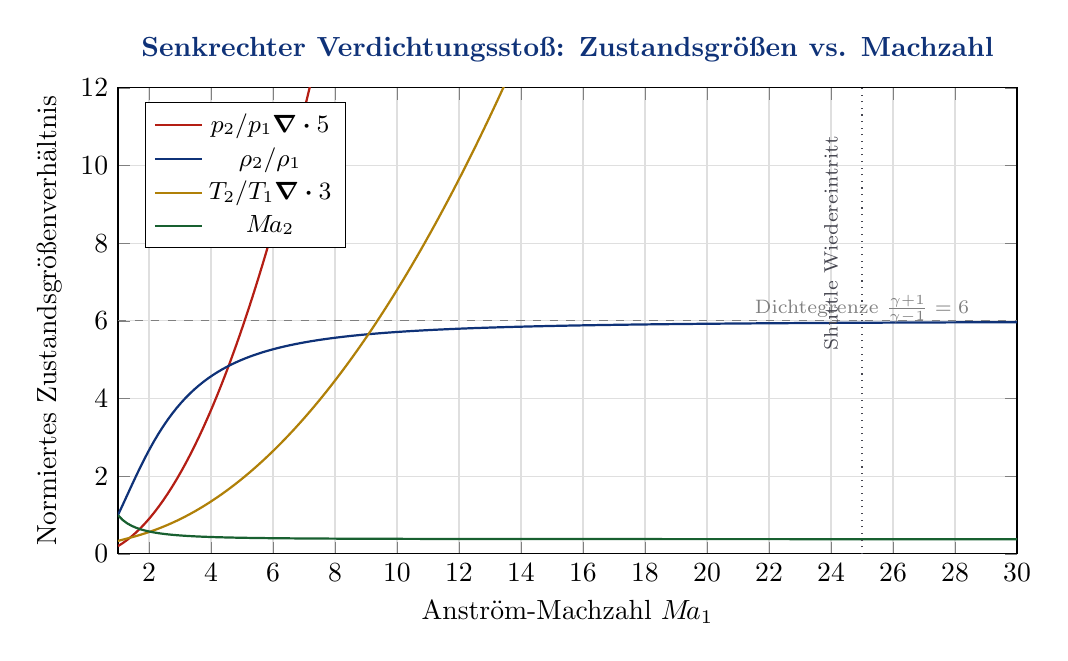
\begin{tikzpicture}
\begin{axis}[
  width=13cm, height=7.5cm,
  xlabel={Anström-Machzahl $\Ma_1$},
  ylabel={Normiertes Zustandsgrößenverhältnis},
  xmin=1, xmax=30,
  ymin=0, ymax=12,
  grid=both, grid style={draw=gray!25},
  title={Senkrechter Verdichtungsstoß: Zustandsgrößen vs. Machzahl},
  title style={font=\normalsize\bfseries\color{hypblau}},
  legend pos=north west, legend style={font=\small},
]
% Druckverhältnis p2/p1 (geteilt durch 20 zur Darstellung)
\addplot[thick, hyprot, domain=1:30, samples=200]
  {(2*1.4*x^2 - (1.4-1))/(1.4+1)/5};
\addlegendentry{$p_2/p_1 \div 5$}

% Dichtesprung rho2/rho1
\addplot[thick, hypblau, domain=1:30, samples=200]
  {(1.4+1)*x^2/((1.4-1)*x^2+2)};
\addlegendentry{$\rho_2/\rho_1$}

% Temperatur T2/T1 / 10
\addplot[thick, schockgelb!80!black, domain=1:30, samples=200]
  {((2*1.4*x^2-(1.4-1))*((1.4-1)*x^2+2)) / ((1.4+1)^2*x^2) / 3};
\addlegendentry{$T_2/T_1 \div 3$}

% Machzahl hinter dem Stoß
\addplot[thick, ablgruen!80!black, domain=1:30, samples=200]
  {sqrt((x^2 + 2/(1.4-1)) / (2*1.4/(1.4-1)*x^2 - 1))};
\addlegendentry{$\Ma_2$}

% Dichtegrenze
\addplot[dashed, gray, domain=1:30] {6};
\node[gray, font=\scriptsize] at (axis cs:25,6.3) {Dichtegrenze $\frac{\gamma+1}{\gamma-1}=6$};

% Markierung Ma=25
\addplot[dotted, dunkelgrau] coordinates {(25,0)(25,12)};
\node[dunkelgrau, font=\scriptsize, rotate=90] at (axis cs:24,8) {Shuttle Wiedereintritt};
\end{axis}
\end{tikzpicture}
\caption{Zustandsgrößensprünge am senkrechten Verdichtungsstoß für $\gamma=1.4$.
Die Dichte nähert sich asymptotisch dem Grenzwert~6, während Druck und Temperatur
quadratisch mit $\Ma$ anwachsen.}
\label{fig:normalstoss}
\end{figure}

\subsection{Schiefer Stoß --- Stoßpolaren (Oblique Shocks)}

Im praktischen Fall trifft eine Strömung auf eine keilförmige Kontur (Rampe,
Nasenspitze). Es entsteht ein schiefer Stoß mit Stoßwinkel $\beta$ bei
Ablenkwinkel $\theta$:

\begin{satz}[Stoßwinkelbedingung ($\theta$-$\beta$-$M$)]
\[
  \tan\theta = 2\cot\beta\cdot
    \frac{\Ma_1^2\sin^2\beta - 1}{\Ma_1^2(\gamma + \cos 2\beta) + 2}
\]
Die Machzahl hinter dem schiefen Stoß:
\[
  \Ma_2^2 = \frac{1 + \frac{\gamma-1}{2}\Ma_1^2}
    {\gamma\Ma_1^2\sin^2\beta - \frac{\gamma-1}{2}}
    + \frac{\Ma_1^2\cos^2\beta}
    {\frac{\gamma-1}{2}\Ma_1^2\sin^2\beta + 1}
\]
\end{satz}

%=======================================================
\section{Aerothermodynamik des Wiedereintritts}
%=======================================================

\subsection{Thermodynamisches Gleichgewicht und Hochtemperatureffekte}

Bei Hyperschallgeschwindigkeiten wird die kinetische Energie des Fahrzeugs durch
die Stoßkompression in thermische Energie umgewandelt. Die dabei erreichten
Temperaturen überschreiten die Dissoziationsenergien molekularer Spezies:

\begin{table}[H]
\centering
\caption{Hochtemperatureffekte in Luft bei steigender Temperatur}
\label{tab:hochtemp}
\begin{tabular}{lrl}
\toprule
\textbf{Phänomen} & \textbf{Temp. [K]} & \textbf{Reaktion}\\
\midrule
Vibrationserregung O$_2$        & 800    & Anregung innerer Freiheitsgrade\\
Vibrationserregung N$_2$        & 1\,000 & Vollständige Vibration aktiv\\
Dissoziation O$_2$              & 2\,000 & $\mathrm{O_2 \to 2\,O}$\\
Dissoziation N$_2$              & 4\,000 & $\mathrm{N_2 \to 2\,N}$\\
Ionisation O, NO                & 9\,000 & $\mathrm{O \to O^+ + e^-}$\\
Ionisation N                    & 14\,000& $\mathrm{N \to N^+ + e^-}$\\
\bottomrule
\end{tabular}
\end{table}

Diese Prozesse \emph{senken} den effektiven Isentropenexponenten $\gamma_{\text{eff}}$
erheblich: Während für kalte Luft $\gamma = 1.4$ gilt, fällt dieser Wert bei
$T > \SI{6000}{K}$ auf $\gamma_{\text{eff}} \approx 1.1\ldots1.2$. Dies hat
gravierende Konsequenzen: Die Dichtegrenze steigt von 6 auf bis zu 12--14.

\begin{herleitung}[Realgaseffekt auf die Dichtegrenze]
Für reales Gas mit effektivem $\gamma_{\text{eff}}$:
\[
  \left.\frac{\rho_2}{\rho_1}\right|_{\Ma\to\infty}
    = \frac{\gamma_{\text{eff}}+1}{\gamma_{\text{eff}}-1}
\]
Vergleich:
\begin{center}
\begin{tabular}{ccc}
\toprule
$\gamma_{\text{eff}}$ & Physik & Dichtegrenze\\
\midrule
1.40 & Kalte Luft, keine Reaktionen     & 6.00\\
1.30 & Vibration aktiv                   & 7.67\\
1.20 & Partielle Dissoziation            & 11.0\\
1.10 & Starke Dissoziation/Ionisation    & 21.0\\
\bottomrule
\end{tabular}
\end{center}
Die \emph{Stoßlage am Bug} eines Wiedereintrittsfahrzeugs ist somit für reales Gas
\textbf{deutlich näher am Körper} als klassisch berechnet.
\end{herleitung}

\subsection{Staupunkttemperatur und Aeroheating}

Die kinetische Enthalpie einer Strömung mit Geschwindigkeit $V_\infty$ wird am
Staupunkt vollständig in Wärme umgewandelt. Im Idealfall (kein Wandwärmestrom):

\[
  h_0 = h_\infty + \frac{V_\infty^2}{2}
  \quad\Rightarrow\quad
  T_{0,\text{ideal}} = T_\infty + \frac{V_\infty^2}{2c_p}
\]

Für den Wiedereintritt aus LEO ($V_\infty = \SI{7800}{m/s}$, $T_\infty = \SI{220}{K}$,
$c_p = \SI{1005}{J/(kg\cdot K)}$):
\[
  T_{0,\text{ideal}} = 220 + \frac{(7800)^2}{2\times1005}
    \approx 220 + 30\,300 \approx \SI{30\,500}{K}
\]

Diese Zahl zeigt, warum Wiedereintrittsfahrzeuge ohne effektiven Wärmeschutz
augenblicklich verdampfen würden. In der Realität werden durch Dissoziation etwa
65\,\% dieser Energie in chemische Energie (statt Wärme) umgewandelt --- ein
enormer ``natürlicher'' Puffer.

\subsubsection{Wärmefluss am Staupunkt nach Fay-Riddell}

Das Fay-Riddell-Modell liefert den konvektiven Wärmefluss am Staupunkt:

\begin{satz}[Fay-Riddell-Formel]
\[
  \dot{q}_s = 0.763\,\Pr^{-0.6}\,
    \left(\rho_e \mu_e\right)^{0.4}
    \left(\rho_w \mu_w\right)^{0.1}
    \sqrt{\left.\frac{\dd u_e}{\dd x}\right|_s}
    \left(h_{0e} - h_w\right)
    \left[1 + (Le^{0.52}-1)\frac{h_D}{h_{0e}}\right]
\]
wobei $\Pr$ die Prandtl-Zahl, $Le$ die Lewis-Zahl, $h_D$ die
Dissoziationsenthalpie und $\dd u_e/\dd x|_s$ den Geschwindigkeitsgradienten
am Staupunkt bezeichnet.
\end{satz}

In vereinfachter Form (Detra-Kemp-Riddell für kugelförmigen Bug):
\[
  \dot{q}_s = 1.83\times10^{-4}\,\frac{1}{\sqrt{R_N}}
    \sqrt{\frac{\rho_\infty}{\rho_{\mathrm{SL}}}}\,
    \left(\frac{V_\infty}{\SI{7924}{m/s}}\right)^{3.15}
    \quad [\si{W/cm^2}]
\]

Dabei ist $R_N$ der Nasenradius in Metern. \textbf{Schlüsselfolgerung}: Ein
größerer Nasenradius reduziert den Wärmefluss erheblich --- dies ist der Grund,
warum Wiedereintrittskapsel eine stumpfe (blunt body) Konfiguration besitzen.

\begin{figure}[H]
\centering
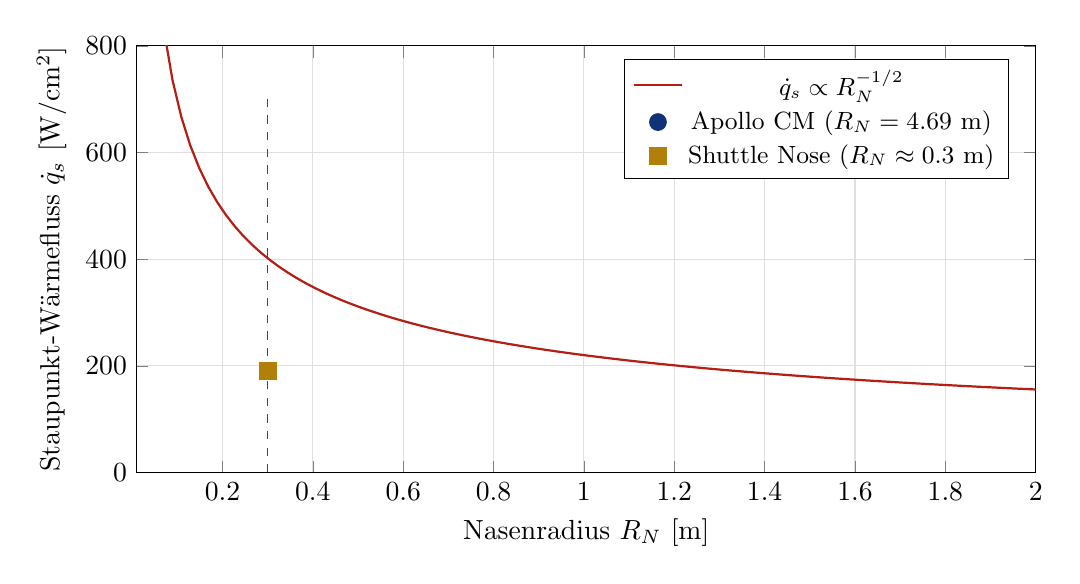
\begin{tikzpicture}
\begin{axis}[
  width=13cm, height=7cm,
  xlabel={Nasenradius $R_N$ [m]},
  ylabel={Staupunkt-Wärmefluss $\dot{q}_s$ [W/cm$^2$]},
  xmin=0.01, xmax=2.0,
  ymin=0, ymax=800,
  grid=both, grid style={draw=gray!25},
  legend pos=north east, legend style={font=\small},
]
\addplot[thick, hyprot, domain=0.05:2.0, samples=100]
  {220/sqrt(x)};
\addlegendentry{$\dot{q}_s \propto R_N^{-1/2}$}

% Markierung Apollo (R=4.7m) -- lit. value ~48 W/cm2
\addplot[only marks, mark=*, mark size=3pt, color=hypblau]
  coordinates {(4.694, 48)};
\addlegendentry{Apollo CM ($R_N=4.69$ m)}

% Markierung Space Shuttle Nose (R=0.3m) -- lit. ~190 W/cm2
\addplot[only marks, mark=square*, mark size=3pt, color=schockgelb!80!black]
  coordinates {(0.3, 190)};
\addlegendentry{Shuttle Nose ($R_N\approx0.3$ m)}

\draw[dashed, dunkelgrau] (axis cs:0.3,0) -- (axis cs:0.3,700);
\draw[dashed, dunkelgrau] (axis cs:4.694,0) -- (axis cs:4.694,700);
\end{axis}
\end{tikzpicture}
\caption{Wärmefluss am Staupunkt nach dem Detra-Kemp-Riddell-Modell bei LEO-Wiedereintritt.
Die stumpfe Bauform der Apollo-Kapsel ($R_N = \SI{4.69}{m}$) reduziert den Wärmefluss
gegenüber der spitzen Shuttle-Nase drastisch.}
\label{fig:waermefluss}
\end{figure}

%=======================================================
\section{Grenzschicht und Wandwärmeübergang}
%=======================================================

\subsection{Hyperschall-Grenzschichttheorie}

Die Grenzschicht bei Hyperschallströmungen weist charakteristische Besonderheiten auf.
Die \emph{viskose Interaktion} beschreibt die starke Kopplung zwischen der
Grenzschicht und der Außenströmung, die durch die Verdichtungswirkung der Grenzschicht
auf die Außenströmung entsteht.

\subsubsection{Adiabate Wandtemperatur (Recovery Temperature)}

Selbst ohne Wärmezufuhr stellt sich an einer isolierten Wand eine sogenannte
Rückgewinnungstemperatur ein:
\[
  T_{\mathrm{aw}} = T_e \left(1 + r\,\frac{\gamma-1}{2}\Ma_e^2\right)
\]
wobei $r$ der Rückgewinnungsfaktor ist: $r = \Pr^{1/2}$ (laminare Grenzschicht)
bzw. $r = \Pr^{1/3}$ (turbulente Grenzschicht), und $\Pr \approx 0.71$ für Luft.

\subsubsection{Stanton-Zahl und Reynolds-Analogie}

Der lokale konvektive Wärmefluss zur Wand:
\[
  \dot{q}_w = St\,\rho_e u_e\,(h_{\mathrm{aw}} - h_w)
\]

Die Stanton-Zahl $St$ verknüpft Wärme- und Reibungsübertragung über die
Reynolds-Colburn-Analogie:
\[
  St \cdot \Pr^{2/3} = \frac{C_f}{2}
\]

Für die laminare Grenzschicht über eine ebene Platte (Blasius/Chapman):
\[
  C_f = \frac{0.664}{\sqrt{Re_x}}, \qquad
  Re_x = \frac{\rho_e u_e x}{\mu_e}
\]

\subsection{Stoß-Grenzschicht-Interaktion}

Ein charakteristisches Phänomen der Hyperschallaerodynamik ist die
\emph{Stoß-Grenzschicht-Interaktion} (Shock-Boundary-Layer Interaction, SBLI).
Wenn ein schiefer Stoß auf eine Grenzschicht trifft, entsteht ein komplexes
Strömungssystem mit möglicher lokaler Ablösung.

\begin{figure}[H]
\centering
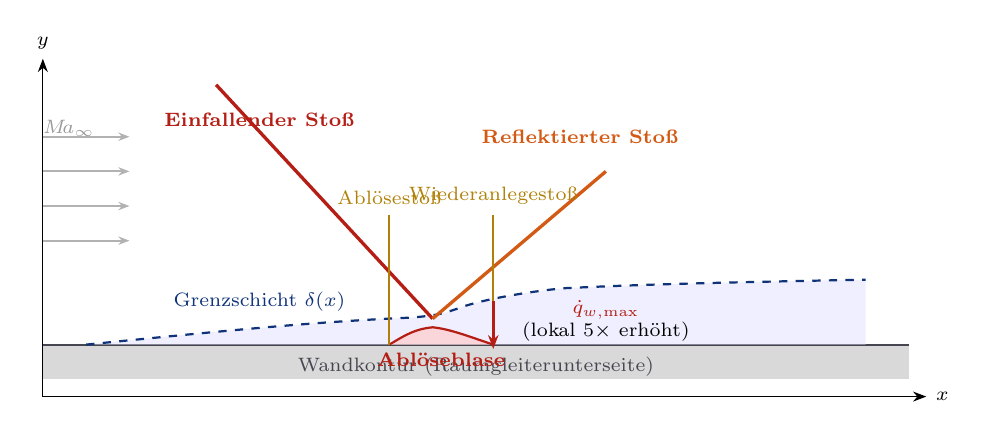
\begin{tikzpicture}[scale=1.1]
  % Wand
  \fill[gray!30] (-1,-0.4) rectangle (9,-0.0);
  \draw[thick, dunkelgrau] (-1,0) -- (9,0);
  \node[font=\scriptsize, dunkelgrau] at (4,-0.25) {Wandkontur (Raumgleiterunterseite)};

  % Grenzschicht (Profil)
  \fill[blue!10, opacity=0.6]
    (-0.5,0) .. controls (1,0.15) and (2,0.25) .. (3,0.30)
    .. controls (3.5,0.32) and (3.6,0.35) .. (3.8,0.42)
    .. controls (4.0,0.5) and (4.5,0.6) .. (5,0.65)
    .. controls (6,0.7) and (7,0.72) .. (8.5,0.75)
    -- (8.5,0) -- (-0.5,0) -- cycle;
  \draw[hypblau, thick, dashed]
    (-0.5,0) .. controls (1,0.15) and (2,0.25) .. (3,0.30)
    .. controls (3.5,0.32) and (3.6,0.35) .. (3.8,0.42)
    .. controls (4.0,0.5) and (4.5,0.6) .. (5,0.65)
    .. controls (6,0.7) and (7,0.72) .. (8.5,0.75);
  \node[hypblau, font=\scriptsize] at (1.5,0.5) {Grenzschicht $\delta(x)$};

  % Anströmung
  \foreach \y in {1.2, 1.6, 2.0, 2.4} {
    \draw[-{Stealth[length=4pt]}, gray!60, line width=0.7pt]
      (-1,\y) -- (0,\y);
  }
  \node[font=\scriptsize, gray!80] at (-0.7,2.5) {$\Ma_\infty$};

  % Einfallender Stoß (von oben)
  \draw[hyprot, very thick] (1.0, 3.0) -- (3.5, 0.30);
  \node[hyprot, font=\scriptsize\bfseries] at (1.5, 2.6) {Einfallender Stoß};

  % Reflexion / Ablösung
  \draw[hitzeorange, very thick] (3.5, 0.30) -- (5.5, 2.0);
  \node[hitzeorange, font=\scriptsize\bfseries] at (5.2, 2.4) {Reflektierter Stoß};

  % Ablöseblase
  \fill[red!20, opacity=0.7]
    (3.0,0) .. controls (3.2,0.12) and (3.3,0.18) .. (3.5,0.20)
    .. controls (3.7,0.18) and (3.9,0.1) .. (4.2,0) -- cycle;
  \draw[hyprot, thick]
    (3.0,0) .. controls (3.2,0.12) and (3.3,0.18) .. (3.5,0.20)
    .. controls (3.7,0.18) and (3.9,0.1) .. (4.2,0);
  \node[hyprot, font=\scriptsize\bfseries] at (3.6,-0.18) {Ablöseblase};

  % Trennlinie / Wiederanlege-Stoß
  \draw[schockgelb!80!black, thick] (3.0,0) -- (3.0,1.5)
    node[above, font=\scriptsize] {Ablösestoß};
  \draw[schockgelb!80!black, thick] (4.2,0) -- (4.2,1.5)
    node[above, font=\scriptsize] {Wiederanlegestoß};

  % Wärmefluss-Spitze (Pfeil)
  \draw[-{Stealth[length=5pt]}, very thick, hyprot]
    (4.2,0.5) -- (4.2,-0.05);
  \node[hyprot, font=\scriptsize\bfseries] at (5.5,0.4) {$\dot{q}_{w,\max}$};
  \node[font=\scriptsize] at (5.5,0.15) {(lokal $5\times$ erhöht)};

  % Koordinaten
  \draw[-{Stealth}] (-1.0,-0.6) -- (9.2,-0.6) node[right, font=\scriptsize] {$x$};
  \draw[-{Stealth}] (-1.0,-0.6) -- (-1.0,3.3) node[above, font=\scriptsize] {$y$};
\end{tikzpicture}
\caption{Stoß-Grenzschicht-Interaktion (SBLI) bei Hyperschall. Der einfallende Stoß
löst die Grenzschicht ab; am Wiederanlegestoß entsteht ein lokales Wärmeflussmaxium,
das den 5-fachen Wert der ungestörten Wandwärme erreichen kann.}
\label{fig:sbli}
\end{figure}

%=======================================================
\section{Wärmeschutzsysteme (Thermal Protection Systems, TPS)}
%=======================================================

Das thermische Schutzsystem ist das kritischste Subsystem jedes Wiedereintrittsfahrzeugs.
Die Auslegung bestimmt Geometrie, Masse und Missionsprofil.

\subsection{Wärmeübertragungsgleichung an der Wand}

Die Energiebilanz an der Außenwand ergibt:
\[
  \rho_s c_s \frac{\partial T}{\partial t}
    = \frac{\partial}{\partial x}\!\left(\lambda_s \frac{\partial T}{\partial x}\right)
    + \dot{q}_{\mathrm{conv}} - \dot{q}_{\mathrm{rad,out}} + \dot{q}_{\mathrm{chem}}
\]

Die \textbf{Strahlungsabgabe} nach außen:
\[
  \dot{q}_{\mathrm{rad,out}} = \varepsilon\,\sigma\,T_w^4
\]
Im Gleichgewicht (Strahlungsgleichgewichtstemperatur):
\[
  \dot{q}_{\mathrm{conv}} = \varepsilon\,\sigma\,T_{w,\mathrm{eq}}^4
  \quad\Rightarrow\quad
  T_{w,\mathrm{eq}} = \left(\frac{\dot{q}_{\mathrm{conv}}}{\varepsilon\,\sigma}\right)^{1/4}
\]

\subsection{Klassifikation der TPS-Konzepte}

\begin{figure}[H]
\centering
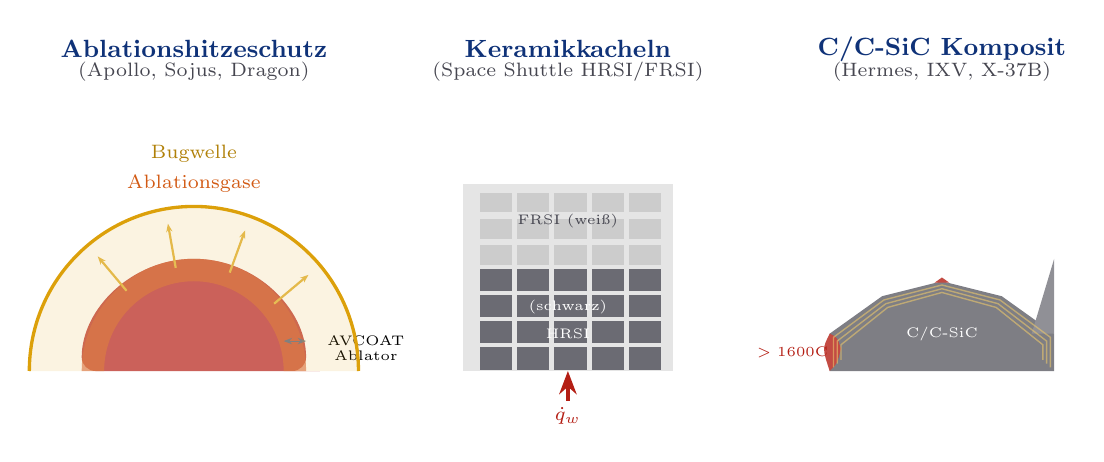
\begin{tikzpicture}[scale=0.95]
  %--- 1: Ablationshitzeschutz (Apollo) ---
  \begin{scope}[xshift=-5cm]
    \node[font=\small\bfseries, hypblau] at (0,4.3) {Ablationshitzeschutz};
    \node[font=\scriptsize, dunkelgrau] at (0,4.0) {(Apollo, Sojus, Dragon)};
    % Kappe
    \fill[hyprot!70, rounded corners=5pt]
      (-1.5,0) arc(180:0:1.5cm) -- (1.5,0) -- cycle;
    % Ablationsschicht (außen)
    \fill[hitzeorange!80, opacity=0.7]
      (-1.5,0) arc(180:90:1.5cm) -- (0,1.5)
      arc(90:0:1.5cm) -- (1.5,0) -- (1.2,0) arc(0:180:1.2cm) -- cycle;
    % Ablationsgase
    \foreach \a in {40,70,100,130} {
      \draw[schockgelb!70, -{Stealth[length=3pt]}, line width=0.8pt]
        ({1.4*cos(\a)},{1.4*sin(\a)}) -- ({2.0*cos(\a)},{2.0*sin(\a)});
    }
    \node[font=\scriptsize, hitzeorange] at (0,2.5) {Ablationsgase};
    % Beschriftungen
    \draw[{Stealth[length=3pt]}-{Stealth[length=3pt]}, gray]
      (1.5,0.4) -- (1.2,0.4) node[midway, right, font=\tiny] {};
    \node[font=\tiny] at (2.3,0.4) {AVCOAT};
    \node[font=\tiny] at (2.3,0.2) {Ablator};
    % Stoßwelle
    \draw[schockgelb, very thick]
      (-2.2,0) arc(180:0:2.2cm);
    \node[schockgelb!80!black, font=\scriptsize] at (0,2.9) {Bugwelle};
    % Heißes Gas
    \fill[schockgelb, opacity=0.12]
      (-2.2,0) arc(180:0:2.2cm) -- (1.5,0) arc(0:180:1.5cm) -- cycle;
  \end{scope}

  %--- 2: Keramikkacheln (Space Shuttle) ---
  \begin{scope}[xshift=0cm]
    \node[font=\small\bfseries, hypblau] at (0,4.3) {Keramikkacheln};
    \node[font=\scriptsize, dunkelgrau] at (0,4.0) {(Space Shuttle HRSI/FRSI)};
    % Rumpf
    \fill[white!80!gray](-1.4,0) rectangle (1.4,2.5);
    % Kachelraster (unten, heiß)
    \foreach \x in {-1.2,-0.7,-0.2,0.3,0.8} {
      \foreach \y in {0,0.35,0.70,1.05} {
        \fill[dunkelgrau!80] (\x+0.02,\y+0.02) rectangle (\x+0.45,\y+0.32);
      }
    }
    % Kachelraster (oben, kühler)
    \foreach \x in {-1.2,-0.7,-0.2,0.3,0.8} {
      \foreach \y in {1.4,1.75,2.1} {
        \fill[white!60!gray] (\x+0.02,\y+0.02) rectangle (\x+0.45,\y+0.28);
      }
    }
    \node[font=\tiny, white] at (0,0.5) {HRSI};
    \node[font=\tiny, white] at (0,0.85) {(schwarz)};
    \node[font=\tiny, dunkelgrau] at (0,2.0) {FRSI (weiß)};
    % Wärmefluss-Pfeil
    \draw[-{Stealth}, hyprot, very thick] (0,-0.4) -- (0,-0.0);
    \node[font=\scriptsize, hyprot] at (0,-0.6) {$\dot{q}_w$};
  \end{scope}

  %--- 3: C/C-SiC (Hermes/IXV) ---
  \begin{scope}[xshift=5cm]
    \node[font=\small\bfseries, hypblau] at (0,4.3) {C/C-SiC Komposit};
    \node[font=\scriptsize, dunkelgrau] at (0,4.0) {(Hermes, IXV, X-37B)};
    % Raumgleiter-Silhouette
    \fill[dunkelgrau!70]
      (-1.5,0) -- (-1.5,0.5) -- (-0.8,1.0) -- (0,1.2) -- (0.8,1.0)
      -- (1.5,0.5) -- (1.5,0) -- cycle;
    % Leitwerk
    \fill[dunkelgrau!60] (1.2,0.5) -- (1.5,1.5) -- (1.5,0.5) -- cycle;
    % Heiße Zonen (Bug + Flügelvorderkanten)
    \fill[hyprot!80]
      (-1.5,0) .. controls (-1.6,0.3) .. (-1.5,0.5)
      .. controls (-1.4,0.45) .. (-1.35,0.3)
      .. controls (-1.4,0.1) .. (-1.5,0) -- cycle;
    \fill[hyprot!80] (-0.1,1.18) -- (0.1,1.18) -- (0,1.25) -- cycle;
    % Isothermen (fake)
    \foreach \s in {0.05,0.1,0.15} {
      \draw[schockgelb!60, line width=0.5pt, opacity=0.6]
        (-1.5+\s,0+\s) -- (-1.5+\s,0.5-\s) -- (-0.8+\s/2,1.0-\s)
        -- (0,1.2-\s) -- (0.8-\s/2,1.0-\s) -- (1.5-\s,0.5-\s) -- (1.5-\s,0+\s);
    }
    \node[font=\tiny, white] at (0,0.5) {C/C-SiC};
    \node[font=\tiny, hyprot] at (-2.0,0.25) {$>1600°$C};
  \end{scope}
\end{tikzpicture}
\caption{Drei Wärmeschutzkonzepte: (links) Einweg-Ablationshitzeschutz der Apollo-Kapsel;
(Mitte) wiederverwendbare Keramikkacheln (HRSI/FRSI) des Space Shuttle;
(rechts) integraler C/C-SiC-Komposit für Raumgleiter.}
\label{fig:tps_vergleich}
\end{figure}

\begin{table}[H]
\centering
\caption{Eigenschaften typischer TPS-Materialien im Vergleich}
\label{tab:tps_mat}
\begin{tabular}{lcccll}
\toprule
\textbf{Material} & $T_{\max}$ [°C] & $\rho$ [kg/m$^3$] &
$\lambda$ & \textbf{Typ} & \textbf{Anwendung}\\
\midrule
AVCOAT 5026-39    & 3\,300 & 512  & 0.25 & Ablator    & Apollo CM, Orion\\
PICA (Phenolic)   & 3\,000 & 260  & 0.14 & Ablator    & Stardust, Dragon\\
LI-900 (HRSI)     & 1\,260 & 144  & 0.05 & Kachel     & Shuttle Unterseite\\
FRCI-12           & 1\,650 & 192  & 0.06 & Kachel     & Shuttle Vorderkante\\
C/SiC Komposit    & 1\,650 & 2\,000 & 8.0 & Strukturell& IXV, X-37B\\
C/C-SiC           & 2\,000 & 1\,800 & 15  & Strukturell& Hermes (konzept.)\\
TUFROC            & 1\,760 & 384  & 0.12 & Hybrid     & X-37B Nase\\
\bottomrule
\end{tabular}
\end{table}

\subsection{Ablationswärmetransfer -- Massenverlustrate}

Beim Ablationshitzeschutz wird Wandmaterial pyrolytisch zersetzt und ausgeblasen.
Die effektive Wärmeschutzmenge ergibt sich aus der Bilanz:
\[
  \dot{m}_{\mathrm{abl}} = \frac{\dot{q}_w - \varepsilon\sigma T_w^4}{h_{\mathrm{eff}}}
\]
wobei $h_{\mathrm{eff}}$ die effektive Pyrolyse-Enthalpie (Sublimationsenthalpie plus
Pyrolyse-Gaskühl\-wirkung) ist. Für AVCOAT: $h_{\mathrm{eff}} \approx \SI{21}{MJ/kg}$.

%=======================================================
\section{Ballistische Eintrittsparameter und Flugmechanik}
%=======================================================

\subsection{Atmosphärisches Eintrittsmodell}

Das vereinfachte Gleichungssystem für einen ballistischen Wiedereintritt
(vernachlässigter Auftrieb, konstante Ballistische Koeffiziente
$\beta_c = m/(C_D A)$) lautet:

\begin{align}
  m\dot{V} &= -\frac{1}{2}\rho(h) V^2 C_D A - mg\sin\gamma
  \label{eq:flugbahn1}\\
  mV\dot{\gamma} &= \frac{1}{2}\rho(h) V^2 C_L A - mg\cos\gamma
    + \frac{mV^2}{r}\cos\gamma
  \label{eq:flugbahn2}\\
  \dot{h} &= -V\sin\gamma
  \label{eq:flugbahn3}
\end{align}

Für ballistischen Eintritt ($C_L = 0$) und exponentielles Atmosphärenmodell
$\rho(h) = \rho_0\,e^{-h/H}$ (Skalenhöhe $H = \SI{7.16}{km}$) lässt sich eine
analytische Näherung für die maximale Verzögerung ableiten:

\begin{herleitung}[Maximalverzögerung beim ballistischen Eintritt]
Chapman (1958) zeigt, dass für $C_L=0$, $\gamma = \text{const}$ (flacher Eintritt):
\[
  \frac{\dd V}{\dd h} = \frac{\rho(h) V C_D A}{2m\sin\gamma}
\]
Die maximale Verzögerung tritt bei der Dichte
$\rho^* = \frac{2m\sin\gamma}{C_D A\,H} = \frac{2\beta_c\sin\gamma}{H}$
auf. Die zugehörige Verzögerung:
\[
  \left|\frac{\dd V}{\dd t}\right|_{\max} = V_e^2\,\frac{\sin\gamma}{2eH}\,\frac{1}{\beta_c/m}
\]
In $g$-Lasten:
\[
  \boxed{n_{\max} = \frac{V_e^2\sin|\gamma_e|}{2\,e\,H\,g_0}}
\]
Für Apollo-Wiedereintritt: $V_e = \SI{11}{km/s}$, $\gamma_e = -6.5°$, $H = \SI{7160}{m}$:
\[
  n_{\max} = \frac{(11000)^2 \times \sin 6.5°}{2\times 2.718\times 7160\times 9.81}
  \approx \frac{1.21\times 10^8\times 0.113}{3.83\times 10^5}
  \approx \mathbf{35.7\,g}
\]
\end{herleitung}

\begin{figure}[H]
\centering
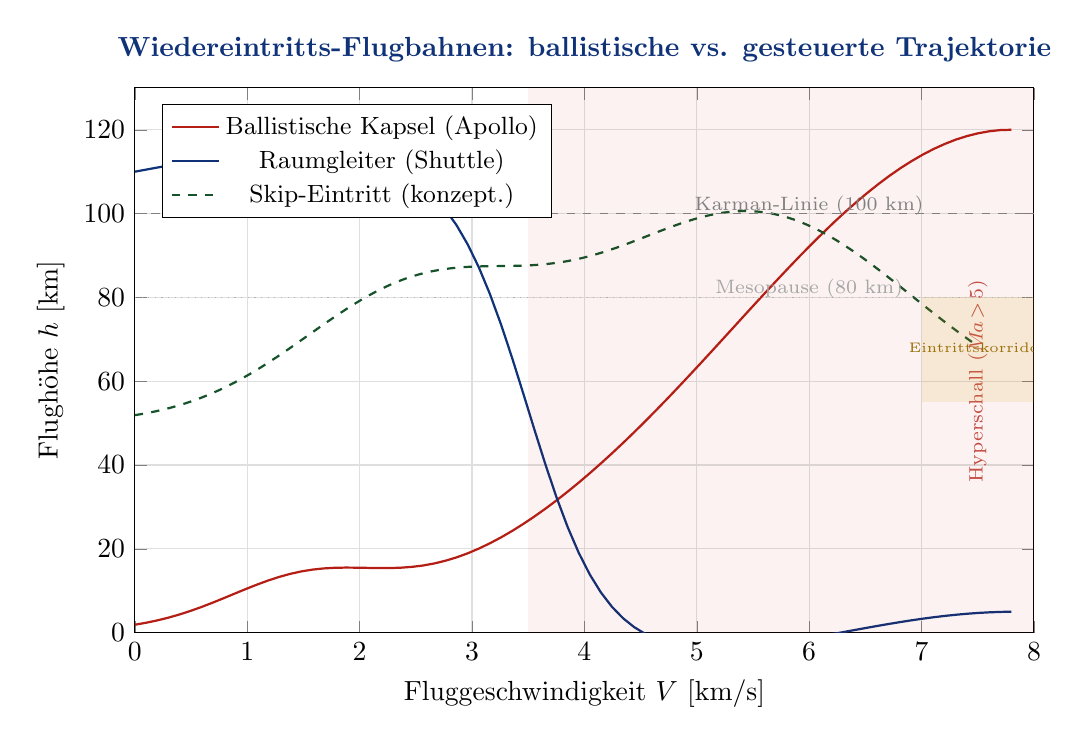
\begin{tikzpicture}
\begin{axis}[
  width=13cm, height=8.5cm,
  xlabel={Fluggeschwindigkeit $V$ [km/s]},
  ylabel={Flughöhe $h$ [km]},
  xmin=0, xmax=8,
  ymin=0, ymax=130,
  grid=both, grid style={draw=gray!25},
  title={Wiedereintritts-Flugbahnen: ballistische vs. gesteuerte Trajektorie},
  title style={font=\normalsize\bfseries\color{hypblau}},
  legend pos=north west, legend style={font=\small},
]
% Ballistische Bahn (Kapsel)
\addplot[thick, hyprot, domain=0:7.8, samples=80]
  {120 - 120*(1 - exp(-((x-7.8)/3.5)^2)) + 10*exp(-((x-1.5)/1.0)^2)};
\addlegendentry{Ballistische Kapsel (Apollo)}

% Gesteuerte Bahn (Raumgleiter)
\addplot[thick, hypblau, domain=0:7.8, samples=80]
  {110 - 110/(1+exp(-3*(x-3.5))) + 5*sin(deg(x))};
\addlegendentry{Raumgleiter (Shuttle)}

% Skip-Wiedereintritt (konzept.)
\addplot[thick, ablgruen!70!black, dashed, domain=0:7.5, samples=120]
  {50 + 50*exp(-((x-5.5)/2.0)^2) + 30*exp(-((x-2.5)/1.5)^2)};
\addlegendentry{Skip-Eintritt (konzept.)}

% Hyperschallbereich
\fill[hyprot, opacity=0.06]
  (axis cs:3.5,0) rectangle (axis cs:8,130);
\node[hyprot!80, font=\scriptsize, rotate=90] at (axis cs:7.5,60) {Hyperschall ($\Ma\!>\!5$)};

% Eintrittskorridore
\fill[schockgelb, opacity=0.12]
  (axis cs:7.0,55) rectangle (axis cs:8.0,80);
\node[schockgelb!70!black, font=\tiny] at (axis cs:7.5,68) {Eintrittskorridor};

% Karman-Linie
\addplot[dashed, gray, domain=0:8] {100};
\node[gray, font=\scriptsize] at (axis cs:6,102) {Karman-Linie (100 km)};

% Thermosphäre
\addplot[dotted, gray!60, domain=0:8] {80};
\node[gray!70, font=\scriptsize] at (axis cs:6,82) {Mesopause (80 km)};
\end{axis}
\end{tikzpicture}
\caption{Vergleich von Wiedereintrittstrajektorien in der Höhen-Geschwindigkeitsebene.
Die ballistische Kapsel folgt einer steilen Bahn mit hoher Spitzenverzögerung;
der Raumgleiter nutzt Auftrieb für einen flacheren, thermisch schonenderen Eintritt.}
\label{fig:trajektorien}
\end{figure}

\subsection{Auftriebskraft und Gleitzahl beim Raumgleiter}

Für einen Raumgleiter mit Auftriebsbeiwert $C_L$ und Widerstandsbeiwert $C_D$
gilt im stationären Gleitflug:
\[
  L = W\cos\gamma, \quad D = W\sin\gamma
  \quad\Rightarrow\quad
  \frac{L}{D} = \cot\gamma = \frac{C_L}{C_D}
\]

Die \emph{Gleitzahl} $L/D$ bestimmt maßgeblich die Manövrierfähigkeit und
Landereichweite des Raumgleiters. Für das Space Shuttle: $L/D \approx 4.5$
(hypersonisch) bis $6.5$ (subsonisch). Hochentwickelte Konzepte wie HL-20 oder
X-38 erreichen $L/D \approx 7$ im Hyperschall.

\subsection{Minimale Entropieproduktion und Entrittskorridorbreite}

Der Eintrittskorridor ist durch zwei Grenzen definiert:

\begin{align}
  \gamma_{\min} &: \quad \text{Überhitzung (zu steiler Eintritt)} \\
  \gamma_{\max} &: \quad \text{Überfliegen / kein Wiedereintritt (zu flach)}
\end{align}

Aus der Wärmeflussbeschränkung $\dot{q}_w \leq \dot{q}_{\max}$:
\[
  |\gamma_e|_{\min} = \arcsin\!\left(\frac{2\,\dot{q}_{\max}^2}{\rho_0\,V_e^3 A_s}\right)
\]

%=======================================================
\section{Zivilfahrzeuge: Konfigurationen und Auslegung}
%=======================================================

\subsection{Stumpfkörper-Kapsel (Blunt Body)}

\begin{figure}[H]
\centering
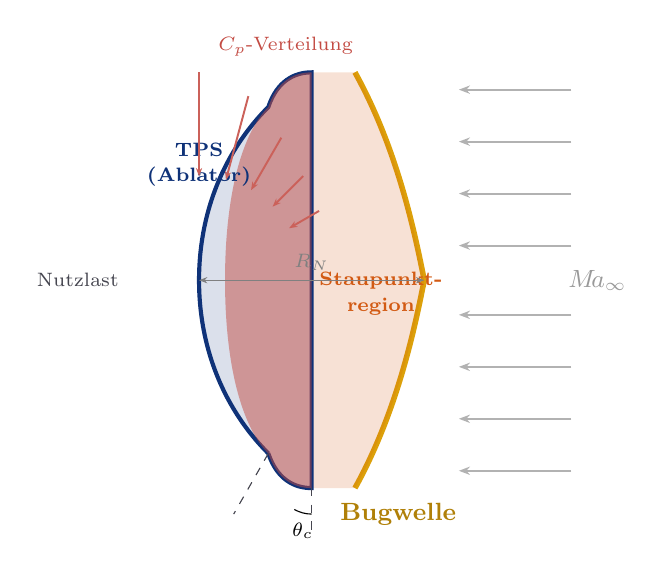
\begin{tikzpicture}[scale=1.1]
  % Strömungspfeile (Anströmung von rechts)
  \foreach \y in {-2.2,-1.6,-1.0,-0.4,0.4,1.0,1.6,2.2} {
    \draw[-{Stealth[length=4pt]}, gray!60, line width=0.7pt]
      (5.5,\y) -- (4.2,\y);
  }
  \node[font=\small, gray!80] at (5.8,0) {$\Ma_\infty$};

  % Stoßwelle (weit vor der Kapsel)
  \draw[schockgelb, very thick, line width=2pt]
    (3.0,-2.4) .. controls (3.5,-1.5) and (3.7,-0.5) ..
    (3.8,0.0) .. controls (3.7,0.5) and (3.5,1.5) .. (3.0,2.4);
  \node[schockgelb!80!black, font=\small\bfseries] at (3.5,-2.7) {Bugwelle};

  % Heißes Gas (zwischen Stoß und Kapsel)
  \fill[hitzeorange, opacity=0.18]
    (3.0,-2.4) .. controls (3.5,-1.5) and (3.7,-0.5) ..
    (3.8,0.0) .. controls (3.7,0.5) and (3.5,1.5) .. (3.0,2.4)
    -- (2.5,2.4) -- (2.0,2.0) -- (2.0,-2.0) -- (2.5,-2.4) -- cycle;
  \node[hitzeorange, font=\scriptsize\bfseries] at (3.3,0) {Staupunkt-};
  \node[hitzeorange, font=\scriptsize\bfseries] at (3.3,-0.3) {region};

  % Kapselkontur (Apollo-typ)
  \fill[hypblau!15]
    (2.0,-2.0) .. controls (2.1,-2.3) and (2.3,-2.4) .. (2.5,-2.4)
    -- (2.5,2.4) .. controls (2.3,2.4) and (2.1,2.3) .. (2.0,2.0)
    .. controls (1.5,1.5) and (1.2,0.8) .. (1.2,0)
    .. controls (1.2,-0.8) and (1.5,-1.5) .. (2.0,-2.0) -- cycle;
  \draw[hypblau, thick, line width=1.5pt]
    (2.0,-2.0) .. controls (2.1,-2.3) and (2.3,-2.4) .. (2.5,-2.4)
    -- (2.5,2.4) .. controls (2.3,2.4) and (2.1,2.3) .. (2.0,2.0)
    .. controls (1.5,1.5) and (1.2,0.8) .. (1.2,0)
    .. controls (1.2,-0.8) and (1.5,-1.5) .. (2.0,-2.0);

  % Ablationsschicht (rot)
  \fill[hyprot!80, opacity=0.5]
    (2.0,-2.0) .. controls (2.1,-2.3) and (2.3,-2.4) .. (2.5,-2.4)
    -- (2.5,2.4) .. controls (2.3,2.4) and (2.1,2.3) .. (2.0,2.0)
    .. controls (1.7,1.7) and (1.5,1.0) .. (1.5,0)
    .. controls (1.5,-1.0) and (1.7,-1.7) .. (2.0,-2.0) -- cycle;

  % Nasenradius
  \draw[{Stealth[length=3pt]}-{Stealth[length=3pt]}, gray]
    (1.2,0) -- (3.8,0) node[midway, above, font=\scriptsize] {$R_N$};

  % Deckwinkel
  \draw[dunkelgrau, dashed]
    (2.5,-2.4) -- (2.5,-2.9);
  \draw[dunkelgrau, dashed]
    (2.0,-2.0) -- (1.6,-2.7);
  \draw (2.5,-2.7) arc(270:240:0.4) node[midway, below, font=\scriptsize] {$\theta_c$};

  % Beschriftungen
  \node[hypblau, font=\scriptsize\bfseries] at (1.2,1.5) {TPS};
  \node[hypblau, font=\scriptsize\bfseries] at (1.2,1.2) {(Ablator)};
  \node[dunkelgrau, font=\scriptsize] at (-0.2,0) {Nutzlast};

  % Druckverteilung (oben)
  \foreach \angle/\plen in {90/1.2, 75/1.0, 60/0.7, 45/0.5, 30/0.4} {
    \pgfmathsetmacro{\xp}{1.2*cos(\angle)+1.2}
    \pgfmathsetmacro{\yp}{1.2*sin(\angle)}
    \pgfmathsetmacro{\xpe}{\xp+\plen*cos(\angle)}
    \pgfmathsetmacro{\ype}{\yp+\plen*sin(\angle)}
    \draw[-{Stealth[length=3pt]}, hyprot!70, line width=0.7pt]
      (\xpe,\ype) -- (\xp,\yp);
  }
  \node[hyprot!80, font=\scriptsize] at (2.2,2.7) {$C_p$-Verteilung};
\end{tikzpicture}
\caption{Querschnitt einer ballistischen Wiedereintrittskapsel (Apollo-Typ).
Die große Nasenradius-Krümmung hält die Bugwelle weit vom Körper und reduziert
den Wärmefluss; die Ablationsschicht (rot) schützt die Struktur.}
\label{fig:kapsel}
\end{figure}

\subsection{Raumgleiter --- Delta-Flügel-Konfiguration}

Raumgleiter wie der Space Shuttle oder das ESA-IXV nutzen Auftrieb für einen
kontrollierten Wiedereintritt mit großer Querreichweite. Die aerothermodynamischen
Anforderungen an verschiedene Fahrzeugzonen unterscheiden sich stark:

\begin{table}[H]
\centering
\caption{Thermische Belastungen am Space Shuttle bei Wiedereintritt ($\Ma=25$)}
\label{tab:shuttle_zonen}
\begin{tabular}{llrrl}
\toprule
\textbf{Zone} & \textbf{TPS-Mat.} & $T_{\max}$ [°C] & $\dot{q}_{\max}$ [W/cm$^2$] & \textbf{Auslegungskriterium}\\
\midrule
Nasenvorderkante   & RCC          & 1\,650 & 60  & Strahlungsgleichgewicht\\
Flügelvorderkante         & RCC          & 1\,430 & 45  & Stoß-Grenzschicht-SBLI\\
Unterseite (heiß)         & HRSI  & 1\,260 & 35  & Wärmeleit. + Strahlung\\
Seitenflächen             & FRCI-12      & 760    & 15  & Konvektion gemäßigt\\
Oberseite (kalt)          & FRSI         & 371    & 5   & Niedrige konv. Heizung\\
\bottomrule
\end{tabular}
\end{table}

%=======================================================
\section{Numerische Simulation: CFD für Hyperschall}
%=======================================================

\subsection{DSMC vs. CFD -- Knudsen-Zahl-Abgrenzung}

Die Gültigkeit der Kontinuumsmechanik-Annahme hängt von der Knudsen-Zahl ab:
\[
  Kn = \frac{\lambda}{L} = \frac{\mu}{\rho\,a\,L}\sqrt{\frac{\pi\gamma}{2}}
\]
wobei $\lambda$ die freie Weglänge und $L$ die charakteristische Länge ist.

\begin{figure}[H]
\centering
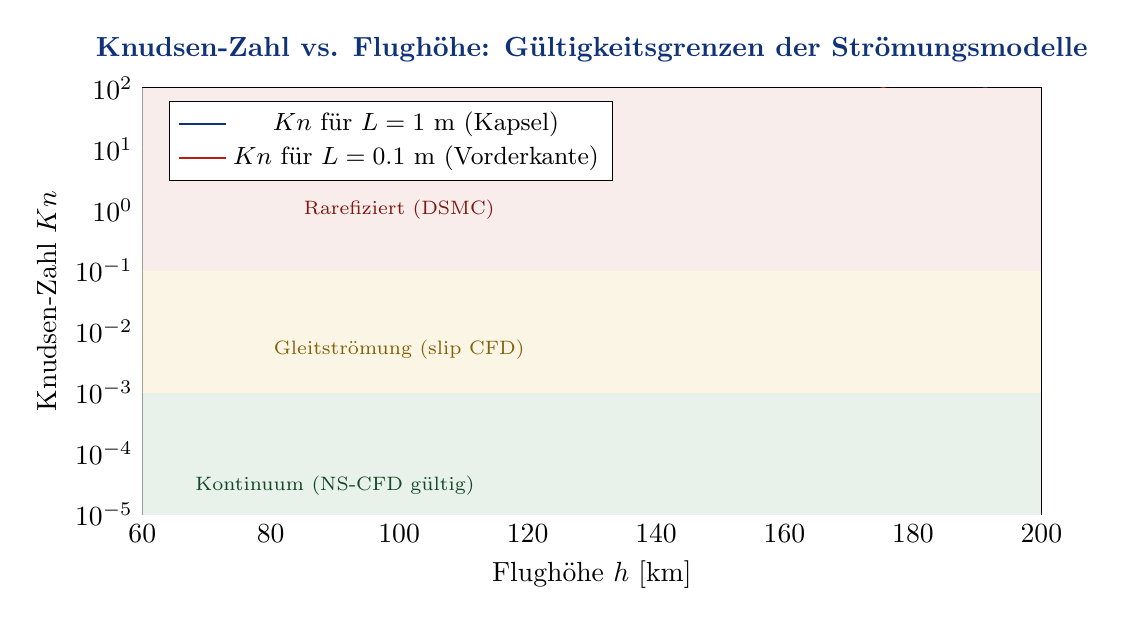
\begin{tikzpicture}
\begin{axis}[
  width=13cm, height=7cm,
  xlabel={Flughöhe $h$ [km]},
  ylabel={Knudsen-Zahl $Kn$},
  xmin=60, xmax=200,
  ymin=1e-5, ymax=100,
  ymode=log,
  grid=both, grid style={draw=gray!25},
  title={Knudsen-Zahl vs. Flughöhe: Gültigkeitsgrenzen der Strömungsmodelle},
  title style={font=\normalsize\bfseries\color{hypblau}},
  legend pos=north west, legend style={font=\small},
]
% Knudsen-Zahl (mittlere freie Weglänge / 1m)
\addplot[thick, hypblau, domain=60:200, samples=100]
  {exp(0.145*(x-80)) * 1e-5};
\addlegendentry{$Kn$ für $L=1$ m (Kapsel)}

\addplot[thick, hyprot, domain=60:200, samples=100]
  {exp(0.145*(x-80)) * 1e-4};
\addlegendentry{$Kn$ für $L=0.1$ m (Vorderkante)}

% Regime-Grenzen
\addplot[dashed, ablgruen!70!black, domain=60:200] {0.001};
\node[ablgruen!70!black, font=\scriptsize] at (axis cs:180,0.0015) {$Kn=0.001$};
\addplot[dashed, schockgelb!80!black, domain=60:200] {0.1};
\node[schockgelb!70!black, font=\scriptsize] at (axis cs:180,0.15) {$Kn=0.1$};
\addplot[dashed, hyprot, domain=60:200] {10};
\node[hyprot, font=\scriptsize] at (axis cs:180,15) {$Kn=10$};

% Beschriftungen der Regimes
\fill[ablgruen!10] (axis cs:60,1e-5) rectangle (axis cs:200,0.001);
\node[ablgruen!60!black, font=\scriptsize] at (axis cs:90,3e-5)
  {Kontinuum (NS-CFD gültig)};
\fill[schockgelb!10] (axis cs:60,0.001) rectangle (axis cs:200,0.1);
\node[schockgelb!60!black, font=\scriptsize] at (axis cs:100,0.005)
  {Gleitströmung (slip CFD)};
\fill[hyprot!8] (axis cs:60,0.1) rectangle (axis cs:200,100);
\node[hyprot!70!black, font=\scriptsize] at (axis cs:100,1.0)
  {Rarefiziert (DSMC)};
\end{axis}
\end{tikzpicture}
\caption{Knudsen-Zahl-Karte als Funktion der Flughöhe. Oberhalb von ca. \SI{90}{km}
(für $L=1$ m) verliert die Kontinuumsmechanik ihre Gültigkeit; dort ist die
Direct Simulation Monte Carlo (DSMC) Methode anzuwenden.}
\label{fig:knudsen}
\end{figure}

\subsection{Turbulenzmodellierung im Hyperschallbereich}

Im Hyperschallbereich gelten besondere Anforderungen an die Turbulenzmodellierung.
Der \emph{Morkovin'sche Skalierungshypothese} zufolge können inkompressible
Turbulenzmodelle für $\Ma < 5$ mit einer Dichteskalierung verwendet werden:

\[
  \tilde{u}_i = \sqrt{\frac{\bar{\rho}}{\rho_\infty}}\, u_i'
\]

Für $\Ma > 5$ versagen Standardmodelle (k-$\omega$, k-$\varepsilon$) aufgrund
von Kompressibilitätskorrektionen und Realgas-Effekten. Empfohlene Modelle:

\begin{itemize}[leftmargin=*]
  \item \textbf{k-$\omega$-SST} mit Sarkar-Dilatationsdissipation für $\Ma < 10$
  \item \textbf{LES} (Large Eddy Simulation) für Transitionsbereiche
  \item \textbf{DSMC} (Direct Simulation Monte Carlo) für rarefizierte Bereiche
  \item \textbf{DSMC-CFD-Hybridmethode} für den Übergangsbereich
\end{itemize}

%=======================================================
\section{Aktuelle Entwicklungen im zivilen Hyperschallbereich}
%=======================================================

\subsection{ESA Intermediate eXperimental Vehicle (IXV)}

Das IXV der ESA demonstrierte 2015 erstmals europäische Wiedereintrittstechnologie
mit einem Lifting-Body-Raumgleiter. Die aerodynamische Konfiguration erreichte
$L/D \approx 0.7$ im Hyperschall --- bewusst konservativ für den ersten Flug.

\subsection{SpaceX Starship -- Belly-Flop Wiedereintritt}

Das Starship-Konzept von SpaceX (ab 2023 in Testflügen) nutzt einen neuartigen
``Bauch-Flop''-Wiedereintritt: Das Fahrzeug tritt mit flachem Körper (hoher $C_D$,
maximale Aerobremsung) ein und dreht sich erst nahe der Landeapproache um.
Die thermische Belastung wird durch eine keramische Kachelmatrix und aktive
Transpirationskühl-(Header-Tank-)Systeme beherrscht.

\subsection{Zusammenfassung: $\Dv$-Budget und Wärmeschutzaufwand}

\begin{figure}[H]
\centering
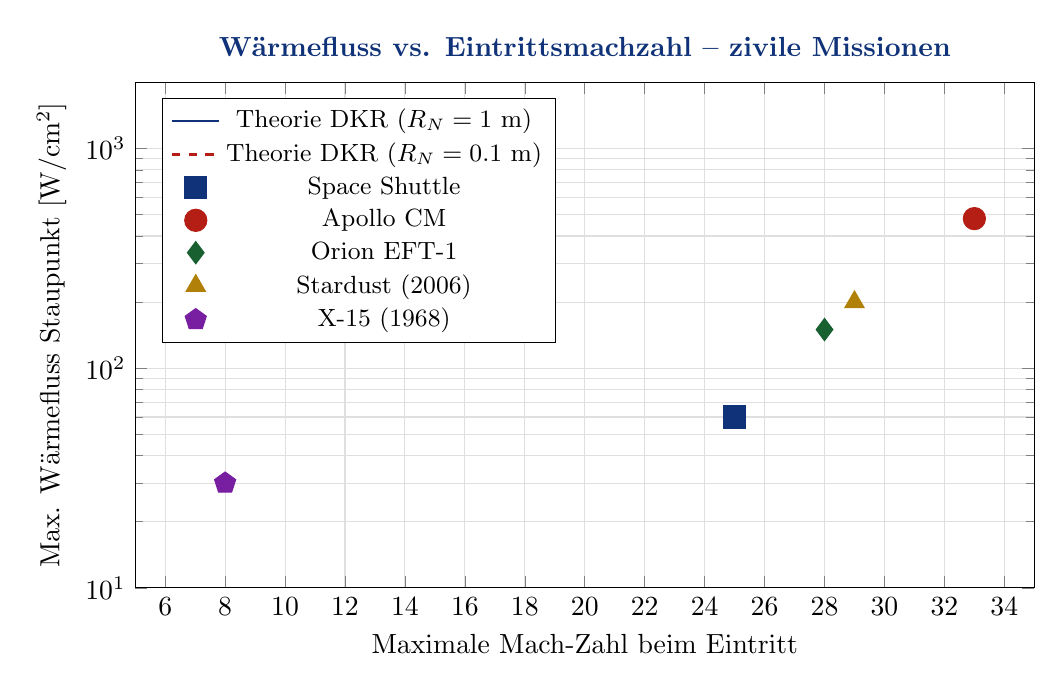
\begin{tikzpicture}
  \begin{axis}[
    width=13cm, height=8cm,
    xlabel={Maximale Mach-Zahl beim Eintritt},
    ylabel={Max. Wärmefluss Staupunkt [W/cm$^2$]},
    xmin=5, xmax=35,
    ymin=10, ymax=2000,
    ymode=log,
    grid=both, grid style={draw=gray!25},
    title={Wärmefluss vs. Eintrittsmachzahl -- zivile Missionen},
    title style={font=\normalsize\bfseries\color{hypblau}},
    legend pos=north west, legend style={font=\small},
  ]
  % Theoretische Kurve (DKR, R_N = 1.0 m, h = 70 km)
  \addplot[thick, hypblau, domain=5:35, samples=100]
    {max(0.1, 1.83e-4/sqrt(1.0) * 0.00894 * ((x * 310)/7924)^3 * 1e4)};
  \addlegendentry{Theorie DKR ($R_N=1$ m)}

  \addplot[thick, hyprot, dashed, domain=5:35, samples=100]
    {max(0.1, 1.83e-4/sqrt(0.1) * 0.00894 * ((x * 310)/7924)^3 * 1e4)};
  \addlegendentry{Theorie DKR ($R_N=0.1$ m)}

  % Reale Fahrzeuge
  \addplot[only marks, mark=square*, mark size=4pt, color=hypblau]
    coordinates {(25,60)};
  \addlegendentry{Space Shuttle}
  \addplot[only marks, mark=*, mark size=4pt, color=hyprot]
    coordinates {(33, 480)};
  \addlegendentry{Apollo CM}
  \addplot[only marks, mark=diamond*, mark size=4pt, color=ablgruen!80!black]
    coordinates {(28, 150)};
  \addlegendentry{Orion EFT-1}
  \addplot[only marks, mark=triangle*, mark size=4pt, color=schockgelb!80!black]
    coordinates {(29, 200)};
  \addlegendentry{Stardust (2006)}
  \addplot[only marks, mark=pentagon*, mark size=4pt, color=plasmaviolett]
    coordinates {(8, 30)};
  \addlegendentry{X-15 (1968)}
  \end{axis}
\end{tikzpicture}
\caption{Maximaler konvektiver Wärmefluss am Staupunkt als Funktion der
Eintrittsmachzahl für reale zivile Missionen, verglichen mit der
Detra-Kemp-Riddell-Theorie bei zwei Nasenradien.}
\label{fig:missionen_vergleich}
\end{figure}

%=======================================================
\section{Schlussbetrachtung}
%=======================================================

Die Hyperschallaerodynamik verbindet fundamentale Strömungsmechanik,
Hochtemperaturphysik, Werkstoffwissenschaft und Regelungstechnik zu einem
der anspruchsvollsten Gebiete der Ingenieurwissenschaften. Drei Kernthemen
beherrschen die Auslegung jedes zivilen Wiedereintrittsfahrzeugs:

\textbf{(1) Thermische Belastung:} Die kinetische Energie eines aus LEO
eintretenden Fahrzeugs übersteigt die Schmelzenthalpie jedes bekannten
Konstruktionswerkstoffs um ein Vielfaches. Nur durch geeignete Geometrie
(stumpfer Bug, großer Nasenradius), fortgeschrittene Materialien (Ablator,
C/C-SiC) und optimierte Trajektorien ist ein sicherer Wiedereintritt möglich.

\textbf{(2) Realgaseffekte:} Für $\Ma > 12$ verliert die Annahme eines
kalorisch perfekten Gases ihre Gültigkeit. Dissoziation und Ionisation senken
den effektiven $\gamma$, verschieben die Stoßlage und verändern die
Wärmeübertragungscharakteristik grundlegend.

\textbf{(3) Kontrollierter Wiedereintritt:} Der Eintrittskorridor ist durch
thermische Constraints nach unten und durch die Notwendigkeit des Atmosphärenfangs
nach oben begrenzt. Raumgleiter mit hoher $L/D$-Zahl können diesen Korridor
aktiv manövrieren; ballistische Kapseln müssen ihn passiv -- durch präzise
Initialbahnausrichtung -- treffen.

\bigskip
\paragraph*{Kernaussagen der Hyperschallaerodynamik}
\begin{itemize}[leftmargin=*]
  \item \textbf{Dichtegrenze}: Am senkrechten Stoß kann sich die Luft maximal
    um den Faktor $(\gamma+1)/(\gamma-1)$ verdichten; für $\gamma=1.4$ ergibt
    das~6; mit Dissoziation bis zu~14.
  \item \textbf{Fay-Riddell}: Wärmefluss am Staupunkt skaliert mit
    $\dot{q}_s \propto R_N^{-1/2}\,V^3$ --- stumpfer Bug ist thermisch günstiger.
  \item \textbf{Realgaseffekte} beginnen bei $T > \SI{2000}{K}$ (O$_2$-Dissoziation)
    und verändern alle aerothermodynamischen Kenngrößen wesentlich.
  \item \textbf{SBLI} (Stoß-Grenzschicht-Interaktion) erzeugt lokale
    Wärmefluss-Spitzen bis zum 5-fachen Wert --- kritisch für Kacheln und
    Vorderkanten.
  \item \textbf{Knudsen-Zahl}: Oberhalb von ca. \SI{90}{km} (für $L\sim$1 m)
    ist Kontinuums-CFD ungültig; DSMC-Methodik erforderlich.
  \item \textbf{Eintrittskorridor}: Zwischen Überhitzungsgrenze (zu steil)
    und atmosphärischem Überfliegen (zu flach) liegt nur ein enger Bereich
    sicherer Eintrittswinkel ($\pm 1\ldots2°$ für Kapseln).
\end{itemize}

%=======================================================
\begin{thebibliography}{9}
%=======================================================

\bibitem{anderson2006}
J.\,D. Anderson:
\textit{Hypersonic and High Temperature Gas Dynamics}.
2.\,Aufl. AIAA Education Series, Reston, 2006.

\bibitem{bertin1994}
J.\,J. Bertin:
\textit{Hypersonic Aerothermodynamics}.
AIAA Education Series, Washington, 1994.

\bibitem{fayriddell1958}
J.\,A. Fay, F.\,R. Riddell:
\textit{Theory of Stagnation Point Heat Transfer in Dissociated Air}.
Journal of the Aeronautical Sciences, 25(2):73--85, 1958.

\bibitem{hirschel2005}
E.\,H. Hirschel:
\textit{Basics of Aerothermodynamics}.
Springer, Berlin, 2005.

\bibitem{gnoffo1999}
P.\,A. Gnoffo:
\textit{Planetary-Entry Gas Dynamics}.
Annual Review of Fluid Mechanics, 31:459--494, 1999.

\bibitem{anderson1989}
J.\,D. Anderson:
\textit{Hypersonic and High Temperature Gas Dynamics -- Introduction to Flight}.
5.\,Aufl. McGraw-Hill, New York, 2005.

\end{thebibliography}

\end{document}
